\chapter{Chef Server}

The Chef Server acts as a hub for configuration data. The server stores cookbooks, the policies that are applied to nodes, and metadata that describes each registered node that is being managed by the chef-client. Nodes use the chef-client to ask the server for configuration details, such as recipes, templates, and file distributions. The chef-client then does as much of the configuration work as possible on the nodes themselves (and not on the server). This scalable approach distributes the configuration effort throughout the organization.

The diagram~\ref{fig:overview_chef_draft} shows the relationships between the various elements of Chef, including the nodes, the server, and the workstations. These elements work together to provide the chef-client the information and instruction that it needs so that it can do its job.

\begin{figure}[ht!]
  \center{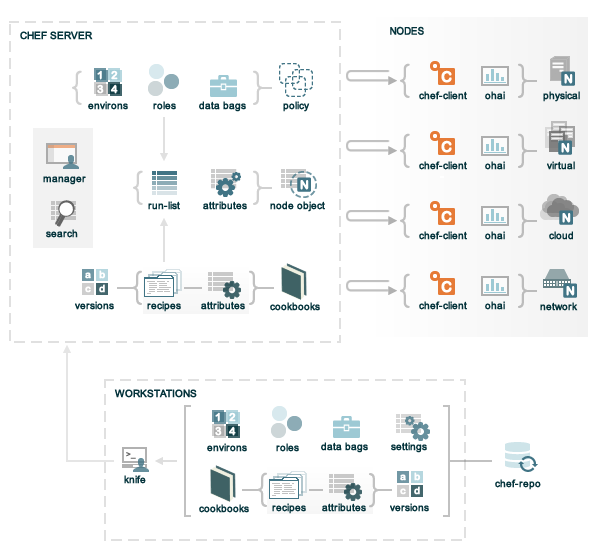
\includegraphics[width=1\textwidth]{overview_chef_draft}}
  \caption{Chef Infrastructure}
  \label{fig:overview_chef_draft}
\end{figure}

We will learn Chef Server by practical examples in this chapter.

\section{Installation}
\label{sec:server-installation}

Exists several ways to install own Chef Server:

\begin{itemize}
  \item Go to \href{http://www.getchef.com/chef/install/}{www.getchef.com/chef/install}, select the operating system, version, and architecture of the server and install the downloaded package on it. After installation you can configure server by command <<sudo chef-server-ctl reconfigure>>
  \item Use Chef Solo to install Chef Server
\end{itemize}

Of course, I prefer to use Chef Solo to install and configure Chef Server. Chef Solo will help us quickly deploy Chef Server on a new server, if something happens with it (crash file system of server, etc.). Do not forget to make a backups of Chef Server (because compared with Chef Solo, Chef Server will be the point of failure in your configuration management system).

Let's create our folder, which will contain all our Chef kitchen:

\begin{lstlisting}[language=Bash,label=lst:my-server-cloud-installation1]
$ mkdir my-server-cloud
$ cd my-server-cloud
$ cat Gemfile
source "https://rubygems.org"

gem 'chef'
gem 'berkshelf'
$ bundle
$ git clone https://github.com/opscode/chef-repo.git .
# or you can use "knife solo init .", if you will install knife-solo
\end{lstlisting}

To install and configure Chef Server exists cookbook \href{https://supermarket.getchef.com/cookbooks/chef-server}{chef-server}. Let's add this cookbook in Berkshelf:

\begin{lstlisting}[label=lst:my-server-cloud-installation2,title=my-server-cloud/Berkshelf]
source "http://api.berkshelf.com"

cookbook 'chef-server'
\end{lstlisting}

After running the command <<berks install>> this cookbook will be installed with dependencies.

\begin{lstlisting}[language=Bash,label=lst:my-server-cloud-installation3]
$ berks install
Installing chef-server (2.0.1) from site: 'http://cookbooks.opscode.com/api/v1/cookbooks'
$ berks install --path cookbooks
Using chef-server (2.0.1)
\end{lstlisting}

Now we should configure a Chef Solo node for our Chef Server. From chapter <<\ref{sec:solo-node}~\nameref{sec:solo-node}>> you should know how to define node.

\begin{lstlisting}[language=JSON,label=lst:my-server-cloud-installation4,title=my-server-cloud/nodes/chef-server.example.com.json]
{
  "fqdn": "10.33.33.33",
  "chef-server": {
    "api_fqdn": "10.33.33.33",
    "version": "latest",
    "configuration": {
      "notification_email": "notify@example.com",
      "chef-server-webui": {
        "enable": true
      }
    }
  },
  "run_list": [
    "recipe[chef-server]"
  ]
}
\end{lstlisting}

By \lstinline!configuration! key you can change settings for Chef Server. All available setting, which can be redefined, you can find \href{https://github.com/opscode/omnibus-chef-server/blob/master/files/chef-server-cookbooks/chef-server/attributes/default.rb}{here}. Our Chef Server by default takes your systems \href{http://en.wikipedia.org/wiki/Fully\_qualified\_domain\_name}{FQDN} as Chef Server url, what is why I set <<fqdn>> in node IP 10.33.33.33, which will set to my server by Vagrant.

First, we should generate Vagrantfile:

\begin{lstlisting}[language=Bash,label=lst:my-server-cloud-installation5]
$ vagrant init precise64
A `Vagrantfile` has been placed in this directory. You are now
ready to `vagrant up` your first virtual environment! Please read
the comments in the Vagrantfile as well as documentation on
`vagrantup.com` for more information on using Vagrant.
\end{lstlisting}

Next we need modeling a cluster of machines by Vagrant. Right now we need only chef server. Let's modify Vagrantfile:

\begin{lstlisting}[label=lst:my-server-cloud-installation6,title=my-server-cloud/Vagrantfile]
# -*- mode: ruby -*-
# vi: set ft=ruby :

require 'chef'
require 'json'

Chef::Config.from_file(File.join(File.dirname(__FILE__), '.chef', 'knife.rb'))

chef_server_json = JSON.parse(Pathname(__FILE__).dirname.join('nodes', 'chef-server.example.com.json').read)

# Vagrantfile API/syntax version. Don't touch unless you know what you're doing!
VAGRANTFILE_API_VERSION = "2"

Vagrant.configure(VAGRANTFILE_API_VERSION) do |config|

  config.vm.define :chef_server do |chef_server|
    chef_server.vm.box = "precise64"
    chef_server.vm.network "private_network", ip: "10.33.33.33"

    chef_server.vm.provision :chef_solo do |chef|
      chef.cookbooks_path = Chef::Config[:cookbook_path]
      chef.roles_path = Chef::Config[:role_path]
      chef.data_bags_path = Chef::Config[:data_bag_path]
      chef.environments_path = Chef::Config[:environment_path]

      chef.run_list = chef_server_json.delete('run_list')
      chef.json = chef_server_json
    end
  end

end
\end{lstlisting}

You should have installed chef gem inside vagrant, as we did in chapter <<\ref{sec:solo-vagrant}~\nameref{sec:solo-vagrant}>> and install/update Chef Client inside server by command <<knife solo prepare>>.

\begin{lstlisting}[language=Bash,label=lst:my-server-cloud-installation7]
$ vagrant provision
[chef_server] Running provisioner: chef_solo...
Generating chef JSON and uploading...
Running chef-solo...
stdin: is not a tty
INFO: Forking chef instance to converge...
INFO: *** Chef 11.8.2 ***
INFO: Chef-client pid: 1831
INFO: Setting the run_list to ["recipe[chef-server]"] from JSON
INFO: Run List is [recipe[chef-server]]
INFO: Run List expands to [chef-server]
...
\end{lstlisting}

We can check Chef Server web interface by \href{https://10.33.33.33}{https://10.33.33.33} and info about libraries version by \href{https://10.33.33.33/version}{https://10.33.33.33/version} url. It should looks like on figure~\ref{fig:chef-server-versions}.

\begin{figure}[ht!]
  \center{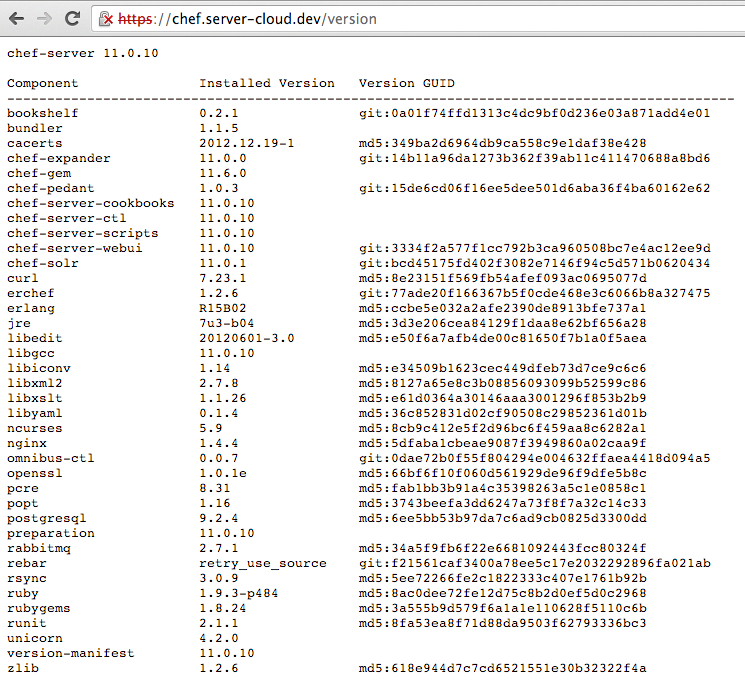
\includegraphics[width=1\textwidth]{chef_server_versions}}
  \caption{Chef Server Versions}
  \label{fig:chef-server-versions}
\end{figure}

I most cases web interface give information about your cloud, which you can get from knife tool. What is why generally it disabled by attribute <<chef-server-webui.enable = false>>.

Next we should configure our knife to work with this Chef Server.

\section{Knife}

After installation Chef Server with default settings, Chef will generate pem keys, which will be used for knife and Chef clients for authentication with server. We should copy its from our Chef Server to <<.chef>> directory in project:

\begin{lstlisting}[language=Bash,label=lst:my-server-cloud-knife1]
$ vagrant ssh chef_server
Welcome to Ubuntu 12.04.1 LTS (GNU/Linux 3.2.0-23-generic x86_64)

vagrant@precise64:~$ sudo cp /etc/chef-server/*.pem /vagrant/.chef/
\end{lstlisting}

On real (production) Chef Server you can use <<scp>> command.

Next we should create for knife configuration file. As you remember from chapter <<\ref{sec:solo-chef-folder}~.Chef folder>>, we already have .chef folder with knife.rb config. But for Chef server we should define additional params. We can use for this <<configure>> command of knife:

\begin{lstlisting}[language=Bash,label=lst:my-server-cloud-knife2]
$ knife configure -i
Overwrite .../my-server-cloud/.chef/knife.rb? (Y/N) y
Please enter the chef server URL: [https://macbookproleo:443] https://10.33.33.33
Please enter a name for the new user: [leo]
Please enter the existing admin name: [admin]
Please enter the location of the existing admin's private key: [/etc/chef-server/admin.pem] .chef/admin.pem
Please enter the validation clientname: [chef-validator]
Please enter the location of the validation key: [/etc/chef-server/chef-validator.pem] .chef/chef-validator.pem
Please enter the path to a chef repository (or leave blank):
Creating initial API user...
Please enter a password for the new user:
Created user[leo]
Configuration file written to .../my-server-cloud/.chef/knife.rb
\end{lstlisting}

Now our file look like this:

\begin{lstlisting}[label=lst:my-server-cloud-knife3,title=my-server-cloud/.chef/knife.rb]
log_level                :info
log_location             STDOUT
node_name                'leo'
client_key               '.chef/leo.pem'
validation_client_name   'chef-validator'
validation_key           '.chef/chef-validator.pem'
chef_server_url          'https://10.33.33.33'
syntax_check_cache_path  '.chef/syntax_check_cache'
\end{lstlisting}

Let's little modify it:

\begin{lstlisting}[label=lst:my-server-cloud-knife4,title=my-server-cloud/.chef/knife.rb]
current_dir = File.dirname(__FILE__)

log_level                :info
log_location             STDOUT
node_name                'leo'
client_key               "#{current_dir}/leo.pem"
syntax_check_cache_path  "#{current_dir}/syntax_check_cache"
validation_client_name   "chef-validator"
validation_key           "#{current_dir}/chef-validator.pem"
chef_server_url          "https://10.33.33.33"
cookbook_path            ["#{current_dir}/../cookbooks", "#{current_dir}/../site-cookbooks"]
node_path                 "#{current_dir}/../nodes"
role_path                 "#{current_dir}/../roles"
data_bag_path             "#{current_dir}/../data_bags"
environment_path          "#{current_dir}/../environments"
#encrypted_data_bag_secret "data_bag_key"

knife[:berkshelf_path] = "cookbooks"
\end{lstlisting}

Let's consider an options (part of this options already considered in chapter <<\ref{sec:solo-chef-folder}~.Chef folder>>):

\begin{itemize}
  \item \textbf{chef\_server\_url} - the URL for the Chef Server
  \item \textbf{node\_name} - the name of the node. This is typically also the same name as the computer from which Knife is run
  \item \textbf{client\_key} - the location of the file which contains the client key. This key used to authenticate with Chef Server
  \item \textbf{validation\_key} - the location of the file which contains the key used when a chef-client is registered with a server. A validation key is signed using the validation\_client\_name for authentication. Default value is <</etc/chef/validation.pem>>
  \item \textbf{validation\_client\_name} - the name of the server that–along with the <<validation\_key>>–is used to determine whether a chef-client may register with a server. The validation\_client\_name located in the server and client configuration files must match
  \item \textbf{syntax\_check\_cache\_path} - all files in a cookbook must contain valid Ruby syntax. Use this setting to specify the location in which Knife caches information about files that have been checked for valid Ruby syntax
  \item \textbf{log\_level} - log level for knife
  \item \textbf{log\_location} - log location for knife
\end{itemize}

Let's check what all works fine:

\begin{lstlisting}[language=Bash,label=lst:my-server-cloud-knife5]
$ knife user list
admin
leo
$ knife client list
chef-validator
chef-webui
\end{lstlisting}

As you can see we successfully get list of users and clients from our Chef Server.
\section{Bootstrap first node}

Once the Chef Server workstation is configured, it can be used to install Chef on one (or more) nodes across the organization using a Knife bootstrap operation. The \inline{knife bootstrap} command is used to SSH into the target machine, and then do what is needed to allow the chef-client to run on the node. It will install the chef-client executable (if necessary), generate keys, and register the node with the Chef Server. The bootstrap operation requires the IP address or FQDN of the target system, the SSH credentials (username, password or identity file) for an account that has root access to the node, and (if the operating system is not Ubuntu, which is the default distribution used by knife bootstrap) the operating system running on the target system.

First, let's add new server in Vagrantfile:

\begin{lstlisting}[label=lst:my-server-cloud-node1,title=my-server-cloud/Vagrantfile]
...

Vagrant.configure(VAGRANTFILE_API_VERSION) do |config|

  ...

  config.vm.define :chef_first_client do |chef_client|
    chef_client.vm.box = "precise64"
    chef_client.vm.network "private_network", ip: "10.33.33.34"
  end

end
\end{lstlisting}

And reload vagrant servers:

\begin{lstlisting}[language=Bash,label=lst:my-server-cloud-node2]
$ vagrant halt chef_server
[chef_server] Attempting graceful shutdown of VM...
$ vagrant up
Bringing machine 'chef_server' up with 'virtualbox' provider...
Bringing machine 'chef_client' up with 'virtualbox' provider...
...
\end{lstlisting}

And now we can bootstrap node:

\begin{lstlisting}[language=Bash,label=lst:my-server-cloud-node3]
$ knife bootstrap localhost -x vagrant -p 2200 -i ~/.vagrant.d/insecure_private_key -N first.example.com --sudo
Bootstrapping Chef on localhost
localhost --2014-01-05 16:01:33--  https://www.opscode.com/chef/install.sh
...
localhost Chef Client finished, 0 resources updated
$ knife node list
first.example.com
\end{lstlisting}

And we can check what node created on server:

\begin{lstlisting}[language=Bash,label=lst:my-server-cloud-node6]
$ knife node list
first.example.com
$ knife client show first.example.com
admin:      false
chef_type:  client
json_class: Chef::ApiClient
name:       first.example.com
public_key: -----BEGIN PUBLIC KEY-----
...
-----END PUBLIC KEY-----

validator:  false
\end{lstlisting}

\subsection{Node in Vagrant}

You can automate registration of node with your Chef Server in Vagrant. Let's add new node in Vagrantfile:

\begin{lstlisting}[label=lst:my-server-cloud-node7,title=my-server-cloud/Vagrantfile]
...

Vagrant.configure(VAGRANTFILE_API_VERSION) do |config|
  ...
  config.vm.define :chef_second_client do |chef_client|
    chef_client.vm.box = "precise64"
    chef_client.vm.network "private_network", ip: "10.33.33.35"
    chef_client.vm.provision :chef_client do |chef|
      chef.chef_server_url = Chef::Config[:chef_server_url]
      chef.validation_key_path = Chef::Config[:validation_key]
      chef.validation_client_name = Chef::Config[:validation_client_name]
      chef.node_name = 'second.example.com'

      chef.delete_node = true
      chef.delete_client = true
    end
  end

end
\end{lstlisting}

As you can see, options for <<chef\_client>> the same as we set in knife.rb. After command \inline{vagrant up} you can check what new node registered:

\begin{lstlisting}[language=Bash,label=lst:my-server-cloud-node10]
$ knife node list
first.example.com
second.example.com
\end{lstlisting}

When you provision your Vagrant virtual machine with Chef server, it creates a new Chef node entry and Chef client entry on the Chef server, using the hostname of the machine. After you tear down your guest machine, Vagrant can be configured to do it automatically with the following settings:

\begin{lstlisting}[label=lst:my-server-cloud-node8]
chef.delete_node = true
chef.delete_client = true
\end{lstlisting}

If you don't specify it or set it to false, you must explicitly delete these entries from the Chef server before you provision a new one with Chef server. For example, using Chef's built-in knife tool:

\begin{lstlisting}[language=Bash,label=lst:my-server-cloud-node9]
$ knife node delete second.example.com
$ knife client delete second.example.com
\end{lstlisting}

And how works cleanup for destroy of server:

\begin{lstlisting}[language=Bash,label=lst:my-server-cloud-node11]
$ vagrant destroy chef_second_client
Are you sure you want to destroy the 'chef_second_client' VM? [y/N] y
[chef_second_client] Forcing shutdown of VM...
[chef_second_client] Destroying VM and associated drives...
[chef_second_client] Running cleanup tasks for 'chef_client' provisioner...
Deleting client "second.example.com" from Chef server...
Deleting node "second.example.com" from Chef server...
$ knife node list
first.example.com
$ knife client list
chef-validator
chef-webui
first.example.com
\end{lstlisting}

As you can see node and client removed from Chef server.

\section{Role}

Role work in the same way, as in Chef Solo (chapter <<\ref{sec:solo-role}~Defining roles>>). For example, we will install on <<first.example.com>> \href{http://community.opscode.com/cookbooks/nginx}{nginx}. First of all, we need add nginx cookbook in Berksfile:

\begin{lstlisting}[label=lst:my-serer-cloud-role1,title=my-server-cloud/Berksfile]
site :opscode

cookbook 'chef-server'
cookbook 'nginx'
cookbook 'yum', '~> 3.0'
\end{lstlisting}

After command \inline{berks install} we will create <<nginx>> role:

\begin{lstlisting}[language=JSON,label=lst:my-serer-cloud-role2,title=my-server-cloud/roles/nginx.json]
{
  "name": "nginx",
  "description": "The base role for systems that serve web server",
  "chef_type": "role",
  "json_class": "Chef::Role",
  "default_attributes": {
    "nginx": {
      "version": "1.4.4",
      "default_site_enabled": true,
      "source": {
        "url": "http://nginx.org/download/nginx-1.4.4.tar.gz"
      },
      "worker_rlimit_nofile": 30000,
      "worker_connections": 4000
    }
  },
  "run_list": [
    "recipe[nginx::source]"
  ]
}
\end{lstlisting}

And <<first.example.com>> node:

\begin{lstlisting}[language=JSON,label=lst:my-serer-cloud-role3,title=my-server-cloud/nodes/first.example.com.json]
{
  "name": "first.example.com",
  "json_class": "Chef::Node",
  "chef_type": "node",
  "normal": {
    "fqdn": "10.33.33.34"
  },
  "default": {},
  "override": {},
  "run_list": [
    "role[nginx]"
  ]
}
\end{lstlisting}

As you can see, node have different format, than Chef Solo. Keys \inline{normal}, \inline{default} and \inline{override} contain attributes. Difference of this attributes you can read in chapter <<\ref{sec:server-attributes}~Attributes>>. Now we should upload cookbooks, role and node in Chef Server. For this we can use knife and berkshelf:

\begin{lstlisting}[language=Bash,label=lst:my-serer-cloud-role4]
// upload all cookbooks from path 'cookbooks' and 'site-cookbooks' (use --force if cookbook frozen).
// But for vendor cookbooks before you need execute 'berks install --path cookbooks'
$ knife cookbook upload -a
// or upload all cookbooks by berks
$ berks upload
// create/update role from file
$ knife role from file roles/nginx.json
// update node from file
$ knife node from file nodes/first.example.com.json
\end{lstlisting}

Next we should can use \inline{knife ssh} command to do something on nodes. The \inline{knife ssh} subcommand is used to invoke SSH commands (in parallel) on a subset of nodes within an organization, based on the results of a search query. Example:

\begin{lstlisting}[language=Bash,label=lst:my-serer-cloud-role5]
// execute on 'first.example.com' chef-client
$ knife ssh 'name:first.example.com' 'sudo chef-client' -i ~/.vagrant.d/insecure_private_key -x vagrant
10.33.33.34 Starting Chef Client, version 11.8.2
10.33.33.34 resolving cookbooks for run list: ["nginx::source"]
...
10.33.33.34 Recipe: nginx::source
10.33.33.34   * service[nginx] action nothing (up to date)
10.33.33.34   * service[nginx] action reload
10.33.33.34     - reload service service[nginx]
10.33.33.34
10.33.33.34 Chef Client finished, 4 resources updated
\end{lstlisting}

After first run of this command next time you can get errors like <<Failed to connect to>>. It is because FQDN set by Ohai in chef-client will not visible hostname (in my example nodes have <<precise64>> hostname). In real cluster you will not have such problems, because you will use real hostnames. But in our case we can use Vagrant <<chef\_client>> stuff. Let's create node <<second.example.com>> and upload it on server:

\begin{lstlisting}[language=JSON,label=lst:my-serer-cloud-role6,title=my-server-cloud/nodes/second.example.com.json]
{
  "name": "second.example.com",
  "json_class": "Chef::Node",
  "chef_type": "node",
  "normal": {
    "fqdn": "10.33.33.35"
  },
  "default": {},
  "override": {},
  "run_list": [
    "role[nginx]"
  ]
}
\end{lstlisting}

\begin{lstlisting}[language=Bash,label=lst:my-serer-cloud-role7]
$ knife node from file nodes/second.example.com.json
\end{lstlisting}

Now you can just run \inline{vagrant provision} for second node:

\begin{lstlisting}[language=Bash,label=lst:my-serer-cloud-role8]
$ vagrant provision chef_second_client
[chef_second_client] Running provisioner: chef_client...
Creating folder to hold client key...
Uploading chef client validation key...
Generating chef JSON and uploading...
[chef_second_client] Warning: Chef run list is empty. This may not be what you want.
Running chef-client...
stdin: is not a tty
INFO: Forking chef instance to converge...
INFO: *** Chef 11.8.2 ***
INFO: Chef-client pid: 1198
...
INFO: Running report handlers
INFO: Report handlers complete
\end{lstlisting}

It will run chef-client on server, which will get all needed info how to <<cook>> node from Chef Server. After this you can check what on url \href{http://10.33.33.35/}{http://10.33.33.35/} running nginx.

\section{Attributes}\label{sec:server-attributes}

An attribute is a specific detail about a node. Attributes are used by the chef-client to understand:

\begin{itemize}
  \item The current state of the node
  \item What the state of the node was at the end of the previous chef-client run
  \item What the state of the node should be at the end of the current chef-client run
\end{itemize}

As you read from previous sections of book, attributes can be defined in node, roles and environments, but it's also can be defined by cookbooks.

\subsection{Attribute Types}

Attribute types can be any of the following:

\begin{itemize}
  \item \textbf{default} - attribute is automatically reset at the start of every chef-client run and has the lowest attribute precedence
  \item \textbf{force\_default} - attribute is used to ensure that an attribute defined in a cookbook (by an attribute file or by a recipe) takes precedence over a default attribute set by a role or an environment
  \item \textbf{normal} - attribute is a setting that persists on the target system and is never reset during a chef-client run. A normal attribute has a higher attribute precedence than a default attribute
  \item \textbf{override} - attribute is automatically reset at the start of every chef-client run and has a higher attribute precedence than default, force\_default, and normal attributes. An override attribute is most often specified in a recipe, but can be specified in an attribute file, for a role, and/or for an environment
  \item \textbf{force\_override} - attribute is used to ensure that an attribute defined in a cookbook (by an attribute file or by a recipe) takes precedence over an override attribute set by a role or an environment
  \item \textbf{automatic} - attribute contains data that is identified by Ohai at the beginning of every chef-client run. An automatic attribute cannot be modified and always has the highest attribute precedence
\end{itemize}

At the beginning of a chef-client run, all default, override, and automatic attributes are reset. The chef-client rebuilds them using data collected by Ohai at the beginning of the chef-client run and by attributes that are defined in cookbooks, roles, and environments. Normal attributes are never reset. All attributes are then merged and applied to the node according to attribute precedence. At the conclusion of the chef-client run, all default, override, and automatic attributes disappear, leaving only a collection of normal attributes that will persist until the next chef-client run.

\subsection{Automatic (Ohai)}

An automatic attribute is a specific detail about a node, such as an IP address, a host name, a list of loaded kernel modules, and so on. Automatic attributes are detected by Ohai and are then used by the chef-client to ensure that these attribute are handled properly during every chef-client run. The most commonly accessed automatic attributes are:

\begin{itemize}
  \item \textbf{node['platform']} - the platform on which a node is running. This attribute helps determine which providers will be used
  \item \textbf{node['platform\_version']} - the version of the platform. This attribute helps determine which providers will be used
  \item \textbf{node['ipaddress']} - the IP address for a node. If the node has a default route, this is the IPV4 address for the interface. If the node does not have a default route, the value for this attribute should be nil. The IP address for default route is the recommended default value
  \item \textbf{node['macaddress']} - the MAC address for a node, determined by the same interface that detects the <<node['ipaddress']>>
  \item \textbf{node['fqdn']} - the fully qualified domain name for a node. This is used as the name of a node unless otherwise set
  \item \textbf{node['hostname']} - the host name for the nod
  \item \textbf{node['domain']} - the domain for the node
  \item \textbf{node['recipes']} - a list of recipes associated with a node (and part of that node’s run-list)
  \item \textbf{node['roles']} - a list of roles associated with a node (and part of that node’s run-list)
\end{itemize}

The list of automatic attributes that are collected by Ohai at the start of each chef-client run vary from organization to organization, and will often vary between the various server types being configured and the platforms on which those servers are run. All attributes collected by Ohai are unmodifiable by the chef-client.

\subsection{Attribute Precedence}

Attribute types can be any of the following:

\begin{enumerate}
  \item A \textbf{default} attribute located in a cookbook attribute file
  \item A \textbf{default} attribute located in a recipe
  \item A \textbf{default} attribute located in an environment
  \item A \textbf{default} attribute located in role
  \item A \textbf{force\_default} attribute located in a cookbook attribute file
  \item A \textbf{force\_default} attribute located in a recipe
  \item A \textbf{normal} attribute located in a cookbook attribute file
  \item A \textbf{normal} attribute located in a recipe
  \item An \textbf{override} attribute located in a cookbook attribute file
  \item An \textbf{override} attribute located in a recipe
  \item An \textbf{override} attribute located in a role
  \item An \textbf{override} attribute located in an environment
  \item A \textbf{force\_override} attribute located in a cookbook attribute file
  \item A \textbf{force\_override} attribute located in a recipe
  \item An \textbf{automatic} attribute identified by Ohai at the start of the chef-client run
\end{enumerate}

where the last attribute in the list is the one that is applied to the node.

Attribute precedence, viewed from the same perspective as the overview diagram~\ref{fig:overview_chef_attributes_precedence}, where the numbers in the diagram match the order of attribute precedence:

\begin{figure}[ht!]
  \center{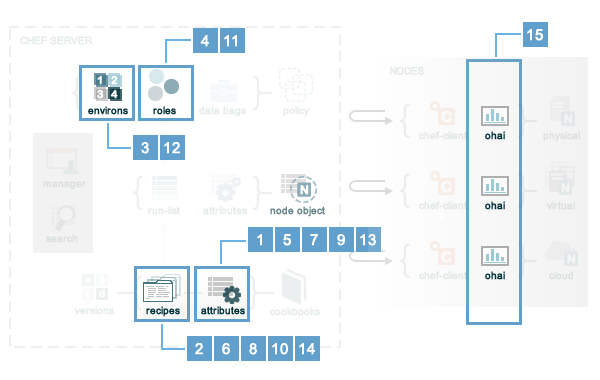
\includegraphics[width=1\textwidth]{overview_chef_attributes_precedence}}
  \caption{Attribute precedence}
  \label{fig:overview_chef_attributes_precedence}
\end{figure}

Attribute precedence~\ref{fig:overview_chef_attributes_table}, when viewed as a table:

\begin{figure}[ht!]
  \center{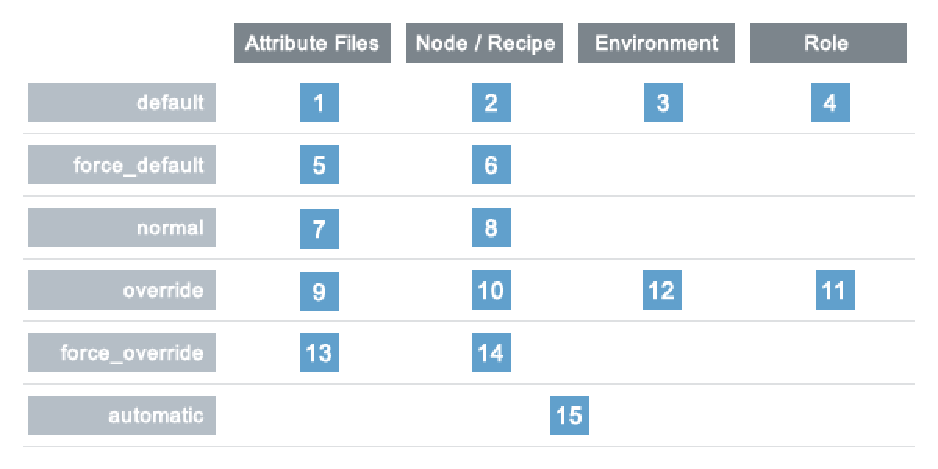
\includegraphics[width=1\textwidth]{overview_chef_attributes_table}}
  \caption{Attribute precedence}
  \label{fig:overview_chef_attributes_table}
\end{figure}
